\documentclass[dvipsnames]{beamer}
 \usepackage{multicol}
 \usepackage{multirow}
 \usepackage{xcolor} 
 \usepackage{graphicx}
 \usepackage{ragged2e}
\usepackage[T1]{fontenc}
\usepackage{helvet}
 
 
 \usepackage{pgfplots}
 \usepackage{pgfplotstable}
 
\usepackage{tikz}
\usetikzlibrary{shapes.geometric, positioning, arrows.meta, decorations.pathreplacing}
\usetikzlibrary{shapes.geometric, arrows}
\definecolor{vino}{rgb}{0.5, 0, 0} 


\setbeamerfont{headline}{size=\fontsize{4}{6}\selectfont}
\useoutertheme[footline=authortitle]{miniframes}



\setbeamercolor{title}{fg=vino}
\setbeamercolor{section in head/foot}{fg=vino} 
\setbeamercolor{subsection in head/foot}{fg=vino} 

\setbeamercolor{frametitle}{fg=vino}
\setbeamercolor{normal text}{fg=black}
\setbeamercolor{item}{fg=black} 

\setbeamerfont{normal text}{size=\fontsize{8pt}{10pt}\selectfont}

%colores
\setbeamercolor{section in toc}{fg=vino}  
\setbeamercolor{subsection in toc}{fg=vino}
%tamño de letra
\setbeamerfont{section in toc}{size=\fontsize{10pt}{14pt}\selectfont} 
\setbeamerfont{subsection in toc}{size=\fontsize{10pt}{14pt}\selectfont}  
%numeración
\setbeamertemplate{section in toc}[sections numbered]   
\setbeamertemplate{subsection in toc}[subsections numbered]   

\setbeamertemplate{itemize items}[circle] 
\setbeamertemplate{itemize subitem}[triangle]




\title[Cámara de refrigeración para insulina en UMF40 Azcapotzalco CDMX]{\textbf{Cálculo y selección de equipo para una cámara de refrigeración para la conservación de insulina en la UMF 40, Santa Bárbara Azcapotzalco CDMX}}
\author{Israel Monjaraz Ramírez\\ 2020360966\\ 9MM1}
\date{9 de diciembre de 2024}

\begin{document}
	\justifying
\begin{frame}
	\thispagestyle{empty}  % Elimina pie de página y encabezado solo en esta diapositiva
	
	
	
	
	\begin{center}
		\begin{footnotesize}		
		\textcolor{vino}{\textbf{Cálculo y selección de equipo}} \\
		\textcolor{vino}{\textbf{para una cámara de refrigeración,}} \\
		\textcolor{vino}{ \textbf{para la conservación de insulina}} \\
		 \textcolor{vino}{\textbf{en la UMF 40, Santa Bárbara} }\\ 
		\textcolor{vino}{ \textbf{Azcapotzalco CDMX}}
	\end{footnotesize}
	\end{center} 
	\begin{minipage}{\textwidth}
		\centering
		\includegraphics[width=0.241108\textwidth]{figures/esimeBN} 	\includegraphics[width=0.241108\textwidth]{figures/ipnlines}  
	\end{minipage}
	
\begin{center}
	\begin{small}
		
	\textcolor{vino}{	\textbf{Israel Monjaraz Ramírez}} \\
	\textcolor{vino}{	\textbf{9 de diciembre de 2024}}  
	\end{small}
\end{center}


\end{frame}

	\section[Contenido]{Contenido de la presentación}
	
\begin{frame}
	\frametitle{Contenido de la presentación}
	\begin{columns}
		\begin{column}{0.5\textwidth}
			\tableofcontents[sections={1-6}]  %, hideallsubsections
		\end{column}
		\begin{column}{0.5\textwidth}
			\tableofcontents[sections={7-12}]
		\end{column}
	\end{columns}
\end{frame}


	% Planteamiento del problema
	\section{Planteamiento}
 
	\justifying
		\fontsize{8}{10}\selectfont
\begin{frame}[plain]
	\frametitle{Planteamiento del problema}
	\justifying
	% Fondo con la imagen
	\begin{tikzpicture}[remember picture, overlay]
		\node[anchor=center] at (current page.center) {
			\includegraphics[width=0.7\paperwidth, height=\paperheight]{figures/diabetes-mx.pdf}
		};
	\end{tikzpicture}
	
	\justifying
	\begin{itemize}[<+->]
		\justifying
		\item \justifying La \textit{diabetes mellitus} es una de las principales causas de muerte en México, con más de 55,000 defunciones reportadas en 2023 (INEGI, 2024).
		\item \justifying Este padecimiento requiere un manejo riguroso de insulina, que debe mantenerse entre 2 °C y 8 °C para garantizar su eficacia.
		\item \justifying La Ciudad de México, principal consumidor nacional de insulina (DataMéxico, 2022), enfrenta retos como el aumento de la temperatura ambiental y fallas en la cadena de frío, que comprometen su estabilidad.
		\item  \justifying En este contexto, se propone diseñar una cámara de refrigeración para la UMF 40 del IMSS, en Azcapotzalco, CDMX, considerando cálculo térmico, selección de equipo y análisis de costos, asegurando la conservación óptima del fármaco para los pacientes atendidos.
	\end{itemize}
\end{frame}

	
	\section{Objetivos}
\begin{frame}
	\frametitle{Objetivos}	
	\fontsize{8}{10}\selectfont
	\justifying	
\subsection{Objetivo general}
\textbf{Objetivo general}\\
Diseñar y calcular una cámara de refrigeración para la conservación de insulina ubicada en la Ciudad de México. 

\subsection{Objetivos específicos}
%\addcontentsline{toc}{section}{Objetivos específicos}
\textbf{Objetivos específicos}\\

\begin{itemize}
	\item	Calcular la potencia, capacidad y carga térmica del sistema. 
	\item	Selección de material aislante térmico bajo las especificaciones obtenidas de la cámara.
	\item	Seleccionar los elementos térmicos para el funcionamiento del sistema frigorífico.
	\item	Diseñar el sistema eléctrico de la cámara de refrigeración. 
	\item	Determinar la capacidad de almacenamiento en función del espacio disponible en la clínica 40 de Azcapotzalco.
	\item	Generar una cámara de dimensiones óptimas comparadas a las del mercado.
\end{itemize}

\end{frame}

\section{Justificación}
	\begin{frame}
		\frametitle{Justificación}
			\justifying	
		El proyecto busca garantizar la conservación óptima de insulina en la UMF 40 de Azcapotzalco, beneficiando a pacientes de la Ciudad de México. Ante el aumento alarmante de casos y muertes por diabetes mellitus en el país, este sistema permitirá mejorar la calidad de vida al asegurar la eficacia del fármaco. Además, se espera que el diseño propuesto funcione eficientemente durante todo el año, especialmente en verano, cuando las temperaturas son más altas, contribuyendo a la estabilidad y seguridad del medicamento.
		
	\end{frame}
	
	% Antecedentes históricos del proyecto
	\section[Antecedentes]{Antecedentes históricos}
\begin{frame}
	\frametitle{Línea de tiempo de la historia de la refrigeración médica}
	\begin{tikzpicture}[xscale=2, yscale=1]
		
		% Timeline axis
		\draw[thick] (0,0) -- (15,0); 
		
		% Events
		\node[anchor=east] at (0,0) {Antigüedad};
		\node[anchor=east] at (3,0) {Grecia y Roma};
		\node[anchor=east] at (6,0) {Época Media};
		\node[anchor=east] at (9,0) {Época Contemporánea};
		\node[anchor=east] at (12,0) {Refrigeración de insulina};
		
		% Event descriptions with blocks
		\node[align=center, fill=blue!20, rounded corners, text width=4cm] at (0,-1.5) {
			La conservación de alimentos en cuevas\\ y el uso de hielo de montaña.
		};
		\node[align=center, fill=yellow!20, rounded corners, text width=4cm] at (3,-1.5) {
			Uso de nieve y hielo para conservar\\ alimentos en climas cálidos.
		};
		\node[align=center, fill=green!20, rounded corners, text width=4cm] at (6,-1.5) {
			Técnicas químicas en la Edad Media\\ para enfriar líquidos y producir hielo.
		};
		\node[align=center, fill=orange!20, rounded corners, text width=4cm] at (9,-1.5) {
			Desarrollo de refrigeración mecánica\\ con experimentos de Cullen y Perkins.
		};
		\node[align=center, fill=purple!20, rounded corners, text width=4cm] at (12,-1.5) {
			Modernización de la refrigeración de la\\ insulina con avances tecnológicos.
		};
		
		% Arrows to the events
		\draw[-{Circle[open]}, thick] (1.2, 0) -- (0.8, 0);
		\draw[-{Circle[open]}, thick] (4.2, 0) -- (3.8, 0);
		\draw[-{Circle[open]}, thick] (7.2, 0) -- (6.8, 0);
		\draw[-{Circle[open]}, thick] (10.2, 0) -- (9.8, 0);
		\draw[-{Circle[open]}, thick] (13.2, 0) -- (12.8, 0);
		
	\end{tikzpicture}
\end{frame}


	\section{Marco teórico}
	\begin{frame}
		\frametitle{Marco teórico} 
		
	\end{frame}
	
 

 	\section[Diseño]{Diseño del sistema solución}
	\begin{frame}
		\frametitle{Diseño del sistema solución}
		
	\end{frame}
	
	\subsection{Criterios de diseño}
\begin{frame}
	\frametitle{Criterios de diseño}
	
\end{frame}



	\subsection[Cálculos]{Cálculos}
	\begin{frame}
		\frametitle{Memoria de cálculo}
		
	\end{frame}
	

	\section[Costos]{Costos del proyecto}
	\begin{frame}
		\frametitle{Costos del proyecto}
		
	\end{frame}

	\section[Conclusión]{Conclusiones}
	\begin{frame}
		\frametitle{Conclusiones}
		
	\end{frame}
	

	\section{Recomendaciones}
	\begin{frame}
		\frametitle{Recomendaciones}
		
	\end{frame}

	\section{Referencias}
	\begin{frame}
		\frametitle{Referencias}
		
	\end{frame}
	

	\section{Fin}
	\begin{frame}
		\frametitle{Fin}
		Muchas gracias por su atención.
	\end{frame}
	
\end{document}
